\subsection{QuizziPedia::Back-End::App}
\subsubsection{Informazioni generali}
\label{QuizziPedia::Back-End::App}
\begin{figure}[ht]
	\centering
	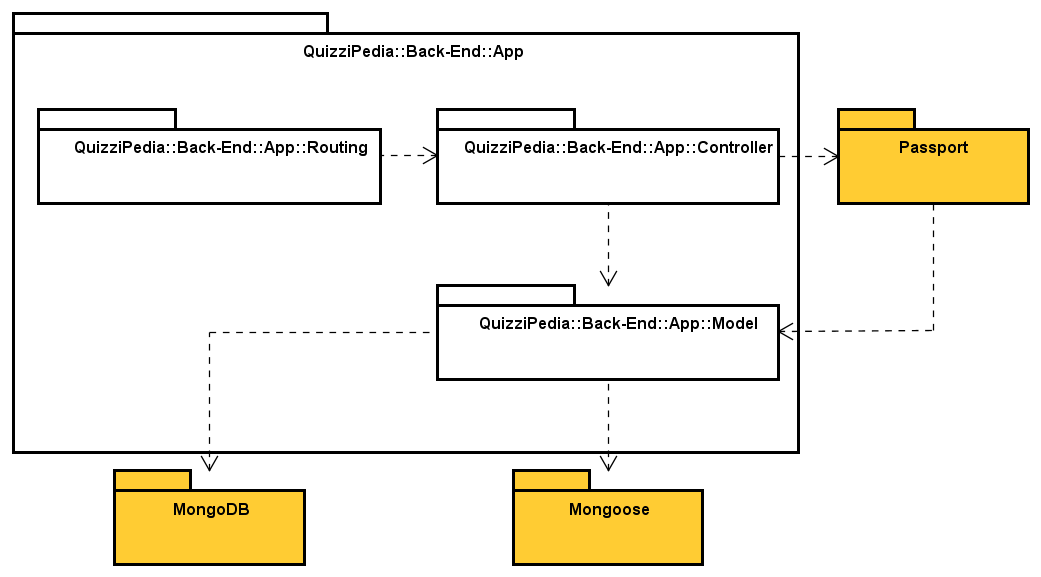
\includegraphics[scale=0.5]{UML/Package/QuizziPedia_Back-End_App.png}
	\caption{QuizziPedia::Back-End::App}
\end{figure}
\FloatBarrier
	\begin{itemize}
		\item \textbf{Descrizione}:
		\textit{package\ped{G}} contenente le componenti del \textit{server\ped{G}} che implementano il \textit{pattern\ped{G} MVC\ped{G}};
		\item \textbf{Padre}: \texttt{Back-End};
		\item \textbf{Interazioni con altri componenti}:
			\begin{itemize}
				\item Config:
				\textit{package\ped{G}} contenente le componenti di configurazione del \textit{server\ped{G}}.
			\end{itemize}
		\item \textbf{Package contenuti}:
			\begin{itemize}
				\item \texttt{Controllers}:
				\textit{package\ped{G}} che contiene i \textit{controllers\ped{G}}  di \textit{Express\ped{G}}, definisce la logica dell'applicazione;
				\item \texttt{Models}:
				\textit{package\ped{G}} che contiene le classi che definiscono il model dell'applicazione. Queste classi cono definite come classi schema di \textit{Mongoose\ped{G}}, il quale permette di utilizzare \textit{MongoDB\ped{G}} tramite degli oggetti;
				\item \texttt{Routers}:
				\textit{package\ped{G}} contenente i \textit{routers} della componente back-end dell'applicazione. Contiene i file di configurazione relativi al routing delle richieste del \textit{client\ped{G}}, ossia i \textit{routers} di \textit{Express\ped{G}}.
			\end{itemize}
	\end{itemize}